\chapter{光照估计数据集的构建与研究}\label{chap:dataset}
%%一种方法是从single-exposure 估计HDR,也可以用来扩充HDR数据集,但是效果不好。
\section{引言}
对于深度学习任务来说,训练数据的规模、质量对网络最终的表现有着直接的影响。小规模的数据、低质量的数据、不平衡的数据都可能会导致网络训练失败。从图片估计光照是一个非常复杂的问题,小规模低质量的数据往往很难训练出较好的预测网络。目前用于光照估计问题的数据集比较有限,主要包括大规模的低动态范围(LDR)全景图和小规模的高动态范围(HDR)全景图。这两类数据集都在规模和质量上,无法同时满足训练一个鲁棒的光照估计网络的条件。因此本文将通过收集、拍摄、筛选、整理等多个严格细致的步骤,构建一个同时包含多类场景的、多种光照条件,而且具有一定规模的光照估计数据集。

本章主要介绍该数据集的构建方式以及在该数据集上的对比试验。本章内容中,首先对低动态范围全景图像和高动态范围全景图像做出介绍;然后阐述HDR全景图的拍摄与合成方法;接着在该数据集上进行多项对比实验,给出了数据集质量和规模对于光照估计问题的影响;最后使用本文数据集与其它多种光照估计数据集进行对比,实验结果验证了本文数据在训练光照估计网络时相对于其它数据的优越性。

本章的主要工作内容和创新点包括:
\begin{itemize}
    \item 深入调研了全景图以及高动态范围全景图的获取步骤、投影方法、存储方式等,并使用全景相机和曝光融合算法构建了一个用于光照估计、大规模、高质量的HDR全景数据集,并通过实验验证了该数据集在光照估计问题中的优越性。
    \item 通过详细的实验分析了HDR全景数据集的规模和多样性对于光照估计问题的影响,证明了丰富的数据多样性和较大的数据规模对深度光照估计表现的有效提升。
\end{itemize}
\section{相关工作}
使用深度学习估计场景光照是近几年光照估计问题的主要研究方向。在深度学习任务中,训练神经网络需要大规模的高质量数据,但目前来说还没有这样的数据在规模和质量上同时满足要求。用于光照估计问题的数据集由两类,分别是规模较大的低动态范围全景数据集和规模较小的高动态范围全景数据集。

规模较大的低动态范围全景数据集以Xiao等人的SUN 360\cite{xiao2012recognizing}为代表。该数据集由26种场景组成,包含了数万张低动态范围的全景图片。数据集中的图片的分辨率为$9104\times4552$。虽然这类数据集的规模较大,但是低动态范围全景图无法直接应用于光照估计,需要使用特定的算法将其转换为粗糙的、低质量的高动态范围全景图,这会对光照估计的结果造成一定影响。

规模较小的高动态范围全景数据集以Gardner等人构建的Laval Indoor\cite{gardner2017learning}为代表。该数据集包含了2100张分辨率为$7768\times3884$的室内高动态范围全景图。拍摄该数据集时,他们将带有Sigma 8mm鱼眼镜头的Canon5D Mark III相机安装在自动的全景机械相机架,并编程拍摄7张不同曝光下的全景图片,这些全景照片以RAW模式拍摄,并使用商业软件PTGui Pro\cite{ptgui}自动拼接和融合为HDR全景图片。该数据集的曝光范围完全能够覆盖真实场景中各个光源的亮度,因此这些数据可以直接应用于光照估计问题中。不过这类数据集的规模通常较小,难以保证训练的效果。

\section{全景图像}
全景图(panorama)是一种广角图,可以以画作、照片、影片、三维模型的形式存在。全景图这个词最早由爱尔兰画家罗伯特·巴克提出,用以描述他创作的爱丁堡全景画。现代的全景图多指通过相机拍摄并在计算机上加工而成的图片\cite{wikipedia}。全景图存储了以相机位置为中心的每个角度的颜色信息,颜色信息与普通图片类似,常用RGB三个通道分别存储。全景图根据其中的颜色数值范围,可分为低动态范围全景图和高动态范围全景图。

\subsection{获取}
拍摄全景图像的方式主要有两类。一类是使用专业的全景相机拍摄设备,这类设备大多由数个鱼眼镜头形式的广角相机组成。在拍摄时,设备中的相机使用相同的相机参数同时拍摄,随后内置的固件或软件会对所拍摄到的图像进行投影变换、校正、拼接,形成一张全景图。另外一类是使用普通相机和相机旋转装置,对多个角度拍摄,随后在手动利用拼接算法或拼接软件将这些图像连接到一起。由于这种方式拍摄到的图片并不在同一个时刻,所以需要保证场景中不能包含过多的快速运动的物体。此外,大多数的现代智能手机都提供了手动拍摄“全景图”的方式。不过需要注意的是,由于相机视角范围限制,以人体为轴旋转手机相机拍摄到的“全景图”多称为“宽景图”,因为顶部视角和底部视角的区域仍然有很大缺失。

\subsection{投影方式}
\begin{figure}[!htbp]
    \centering
    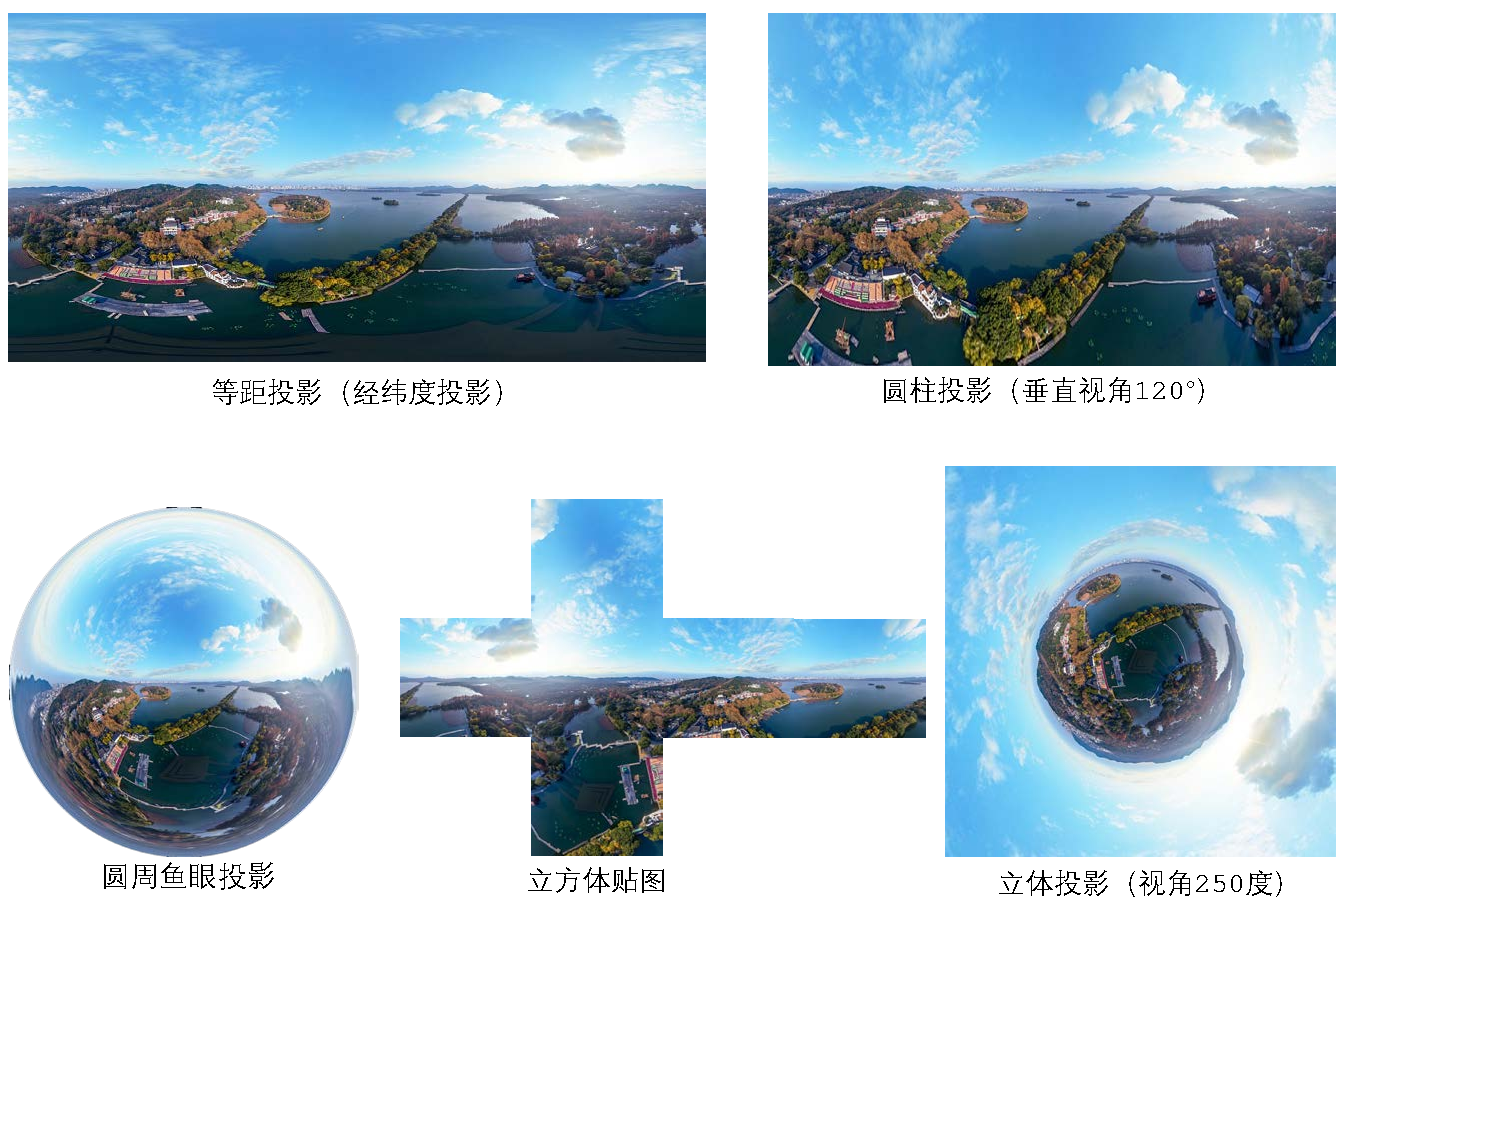
\includegraphics[width=1.0\textwidth]{Img/panorama-projection.pdf}

    \caption[全景图的几种投影方式]
    {
        \label{fig:panorama-projection}
        全景图几种投影方式。等距投影是常见的全景图投影方式,包括了所有视角的信息。圆柱投影的特点致使它不可能有180\doge的垂直视角;圆周鱼眼投影可以显示出所有视角的信息,但是从中可以看到,靠近圆形边缘的区域被极度扭曲,这会因为计算误差导致精度的损失;立方体贴图是计算机图形学中常用的投影方式;立体投影方式看起来像一颗星球,因此也被成为小行星投影方式,这种方式也无法展示所有视角的信息。
    }
\end{figure}
全景图像的存储需要考虑投影方式和颜色的数值类型。在全景图像中,以相机为中心的视场可以被视为一个球体的表面,因此在存储和浏览全景图时,需要将全景球表面投影在二维表面中。常见的投影方式有等距投影,圆柱投影,球形投影,立方体贴图投影,立体投影等。
\begin{itemize}
\item \textbf{圆柱投影}(cylindrical projection)该投影方式是将全景球置于其外切圆柱内,并由球心向圆柱面做投影,随后将圆柱内表面横向展开后的图像即为球形全景图的圆柱投影。这种投影下的全景图在两极会发生无限的纵向拉伸,因此圆柱投影后的图像无法包含靠近两极的信息,也即这种投影方式无法表示垂直视角为180\doge的全景图。柱面投影是传统摆动镜头全景胶片相机所提供的标准投影方式。相对于全角度的全景图,该投影方式更适合在垂直视角小于120\doge的宽景图,常用于现代智能手机的全景图预览。
\item \textbf{等距投影}(equirectangular projection), 也称等距圆柱投影。该投影方式是将球面的经度和纬度坐标线性变换为图像空间的横纵坐标。经过投影处理后的全景图像是一幅宽高比例为2:1的图片。这种投影的特点是越接近两级,图像的变形就越严重。投影后的全景图在预览时一目了然,而且这种投影方式较为简单,是存储和预览全景图最常见的方式之一。
\item \textbf{圆周鱼眼投影}(circumferential fisheye projection),也称圆形投影或镜面球投影,为角投影的一种。这样的投影图像看起来像一个用超级圆形鱼眼镜头所拍摄的图片,虽然这种投影方式依然覆盖360\doge的视角,但是其边缘却被极端扭曲和变形。这种投影方式常见于全景图拍摄设备中。全景相机一般由两个朝向相反的180\doge视角鱼眼镜头。每个镜头所拍摄到的图片均为一个垂直和水平视角各180\doge的圆周鱼眼投影视图。
\item \textbf{立方体贴图投影}(cubemap projection)在计算机图形学中,立方体投影是常用的环境映射方法之一,常用于游戏场景中的天空盒,相当于等距柱状投影的优化版,环境投影到立方体之后可分六个正方形纹理来存储;或者将立方体展开,存储于一个纹理中的六个区域内。 
在全景图像及视频中,立方体投影将球形视频映射到它的外接立方体上,立方体的上下两个面分别对应两极区域,中间的四个面对应赤道区域。
\item \textbf{立体投影} (stereographic projection),这种投影方式常见于一些全景图应用中,因为预览效果类似一颗行星表面,因此也被称为小行星投影。
\end{itemize}
除此之外,还有墨卡托投影、正弦投影等、直线投影用于不同的领域。图\ref{fig:panorama-projection}展示了几种常见的投影方式下的全景图。

\subsection{动态范围}
\begin{figure}[H]
    \centering
    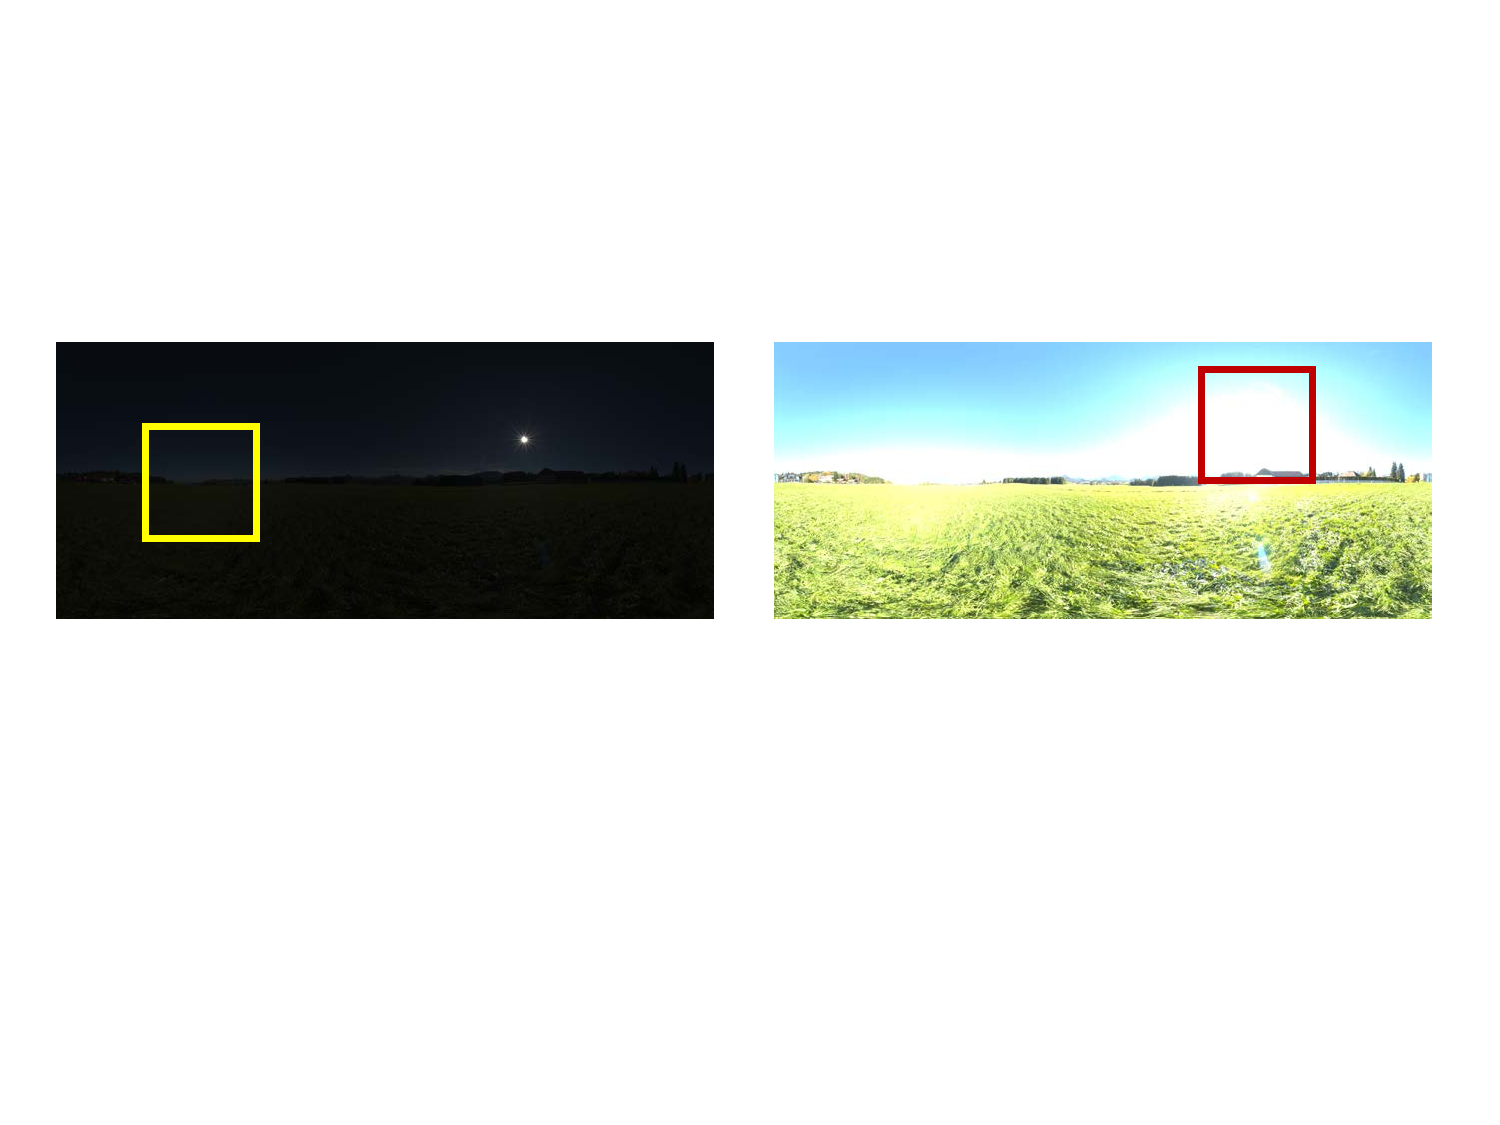
\includegraphics[width=1.0\textwidth]{Img/different-exposure.pdf}
    \caption[使用不同曝光拍摄的LDR图像]
    {两种不同曝光条件下的LDR图像。在欠曝图像中,黄色框选区域中大部分像素均为黑色,但它们的明暗程度并不同;类似地,在过曝图像中,红色框选区域中像素值均为白色,但实际上太阳所处像素的亮度远远高于周围像素。使用LDR图像难以解决这些问题。}
    \label{fig:different-exposure}
\end{figure}
图像的动态范围(dynamic Range)是指一个图像中最亮和最暗部分之间的相对比值\cite{wikipedia}。
根据动态范围的大小可以将图像分为低动态范围(或称为标准动态范围)图像和高动态范围图像。
传统的8位图像将颜色值存储为[0, 255]范围内的整数,低动态范围图像中的颜色只能在这256个数中取值。图\ref{fig:different-exposure}展示了两种不同曝光条件下的照片,可以看出每幅图片都有一定的过曝和欠曝区域。例如在过曝图片中,太阳和其周围区域的颜色均为白色,但实际上太阳的亮度要远远高过天空的亮度;同样的,在欠曝区域中,虽然大部分区域同为黑色,但实际上这些区域的明暗程度也是千差万别的。

\begin{figure}[htbp]
    \centering
    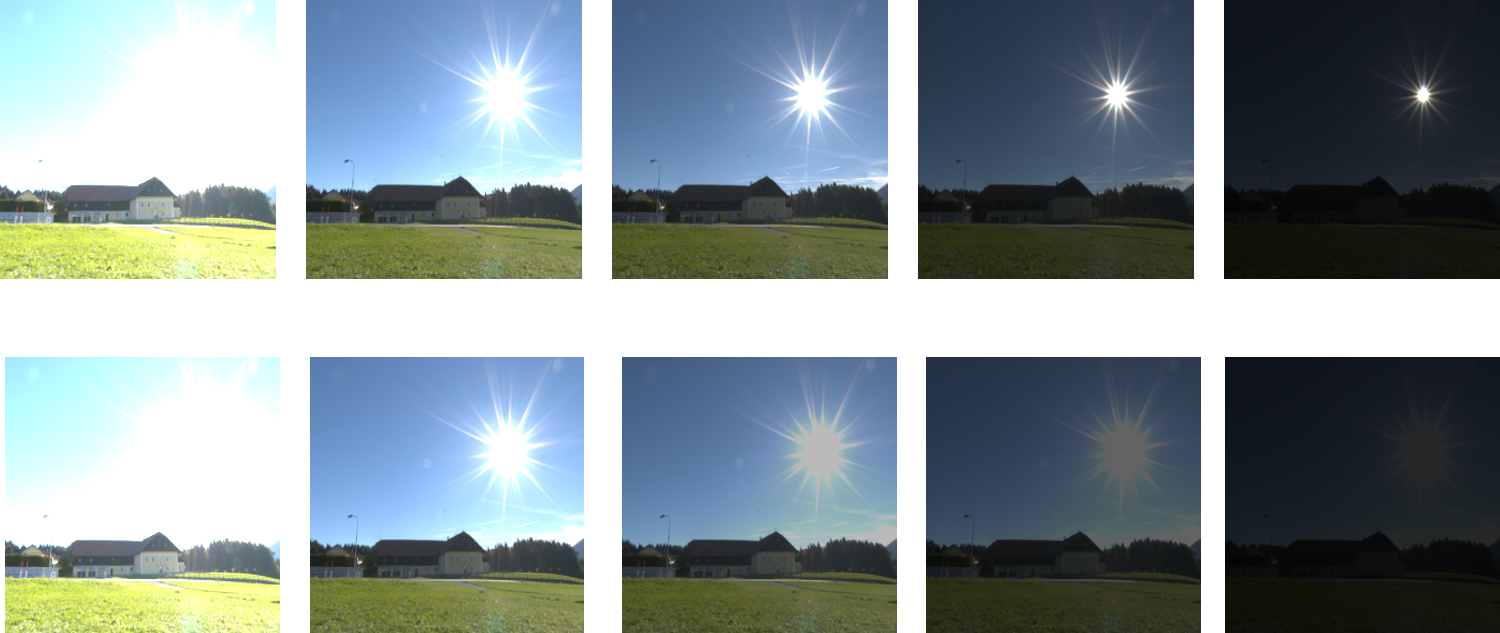
\includegraphics[width=1.0\textwidth]{Img/exposure-change.png}
    \caption[LDR图片与HDR图片在调整曝光时的不同]
    {调整LDR和HDR图像曝光的结果。第一行是从一幅HDR开始,不断减小场景曝光值;第二行则是对LDR执行同样的操作。可以看出对于HDR图像,多次降低曝光后,太阳位置的亮度依然很亮,这说明HDR图像中太阳对应的像素值远远高于周边像素,与真实场景的光照情况一致。而LDR图像在降低曝光后,太阳位置的像素值会和周围像素一起降低,这显然是不符合真实光照条件的。}
    \label{fig:exposure-change}
\end{figure}
而相比低动态范围的图像,高动态范围图像可以提供更多的动态范围(理论上是0到无限大)。图\ref{fig:exposure-change}展示了调整LDR和HDR图像曝光值时的不同点。高动态范围全景图也是具有这种动态范围的全景图像。高动态范围全景图的动态范围可以高达$2^{32}$,而人类的眼睛所能看到的范围是$10^5$左右\cite{wikipedia}。因此高动态范围全景图像可以作为真实的光照信息,这是低动态范围全景图不能比拟的。

\begin{figure}[!htbp]
    \centering
    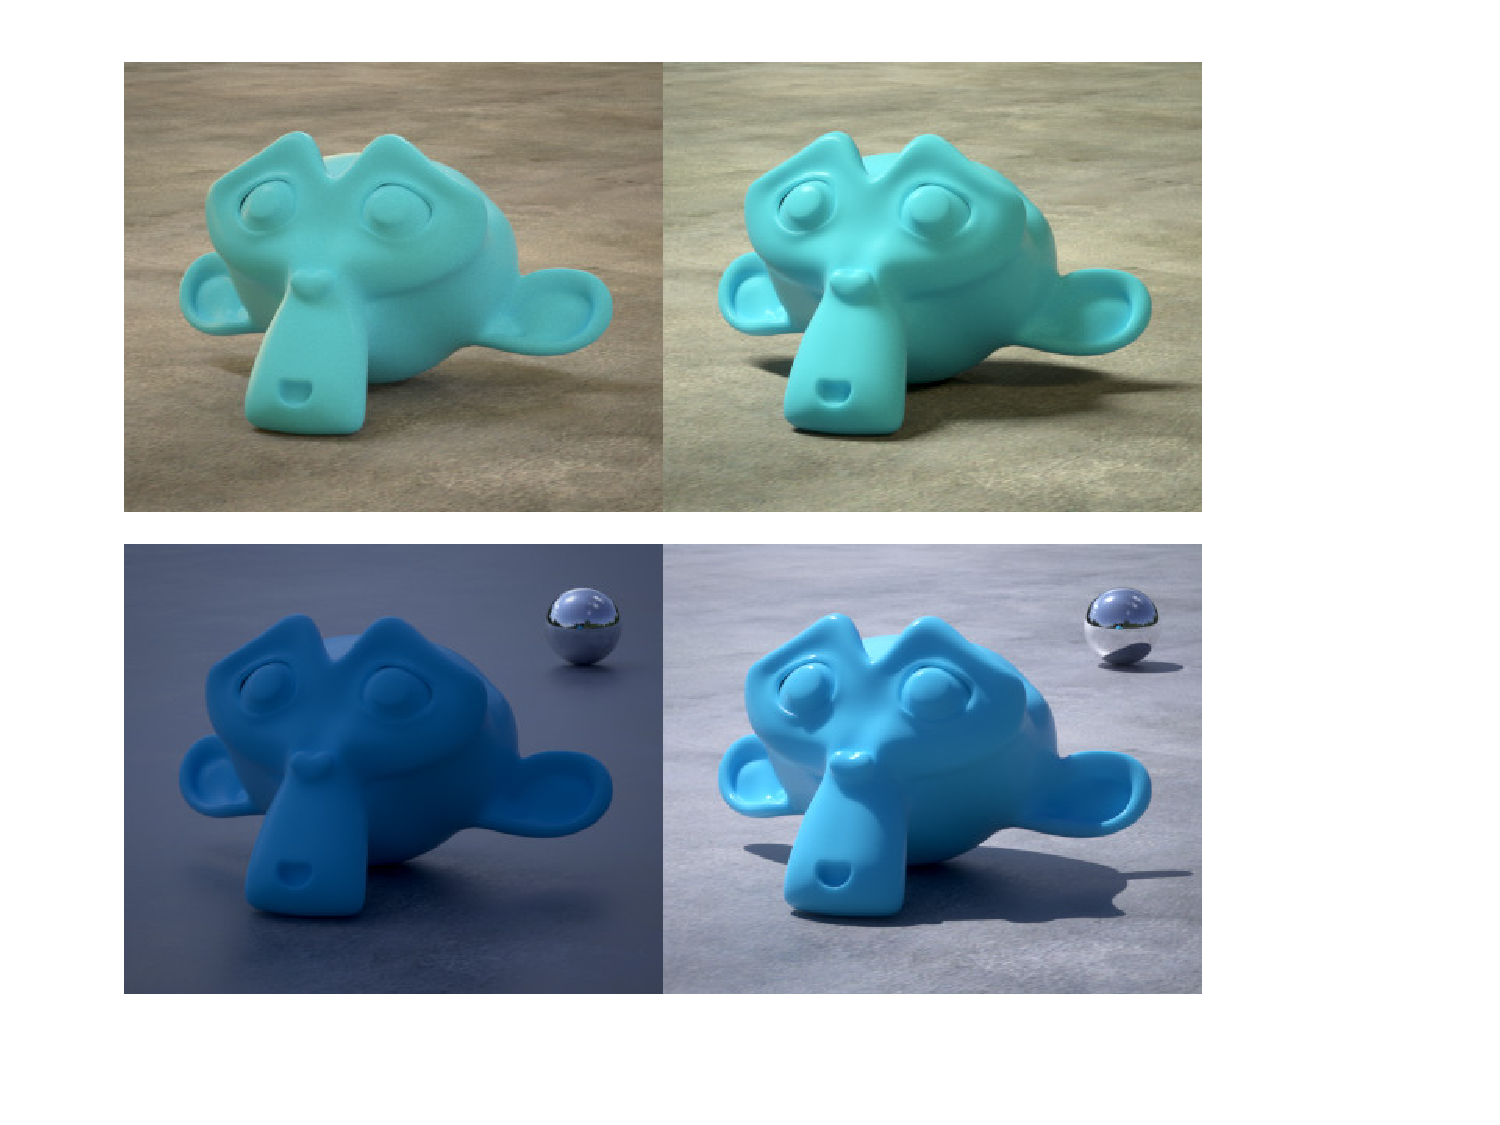
\includegraphics[width=1.0\textwidth]{Img/hdr-render.pdf}
    \caption[使用HDR全景图与LDR全景图渲染结果的对比]
    {使用LDR全景图(左)与使用HDR全景图(右)渲染结果的对比,引自\cite{makehdr}。从第一行可以看出,使用低动态范围全景图像渲染的结果,在颜色上对比平缓,看起来很不真实。而使用HDR全景图渲染的结果提供了足够的对比度和锐利的阴影,更具有真实感。这种情况在场景中有较强光线时尤为明显(第二行结果)}
    \label{fig:hdr-render}
\end{figure}

图\ref{fig:hdr-render}展示了两组使用低动态范围全景图和高动态范围全景图的渲染结果,可以看出,使用低动态范围全景图渲染的结果颜色值对比平缓,看起来很不真实。而使用高动态范围全景图作为光照时,渲染结果包含了足够的对比度和锐利的阴影。图\ref{fig:hdr-render}中的第二行使用了包含更亮光源的场景作为对比,它们之间的差异更加明显。
为方便叙述和浏览,下文中的LDR将代指低动态范围全景图,HDR将代指高动态范围全景图。

\subsection{HDR的获取与存储}
\begin{figure}[!htbp]
    \centering
    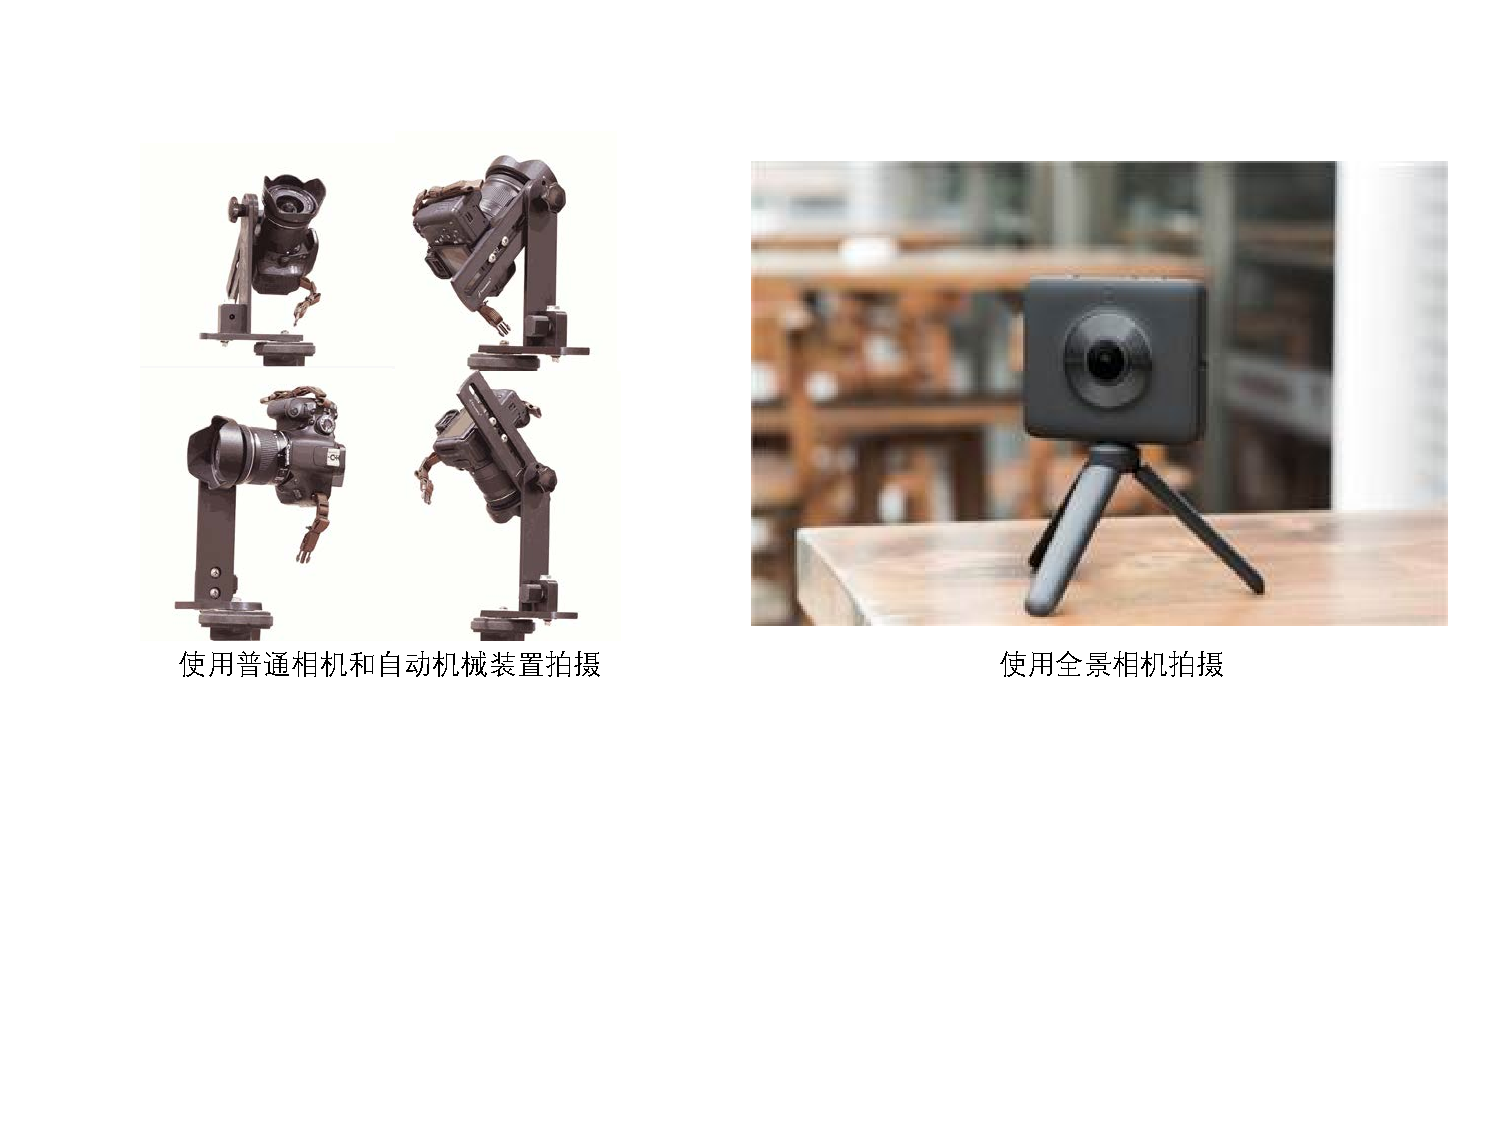
\includegraphics[width=1.0\textwidth]{Img/capture-panorama.pdf}
    \caption[拍摄全景图的示例]
    {常见的拍摄全景图的方式。左图是将单反相机固定在能够自动控制旋转的机械架上,对多个方向进行拍摄,最后利用电脑软件将其拼接到一起;右图是使用全景相机拍摄,由于鱼眼镜头和内置硬件的帮助,这种拍摄方式十分简便,只需一次拍摄就可以获得整个全景图。}
    \label{fig:capture-panorama}
\end{figure}
HDR全景图的获取方式与普通全景图类似,不过由于HDR包含了更大的动态范围。而普通相机单词拍摄无法满足这个要求,因此需要使用对每个视角的图像都要使用不同的曝光值来进行拍摄。
HDR全景图的获取分为多曝光拍摄,多视角拍摄,全景图拼接,清洗和筛选,曝光融合五个步骤。
\begin{itemize}
    \item \textbf{多曝光拍摄}。HDR图像通常无法直接由拍摄设备直接获取,因此需要利用不同的曝光值对同一场景多次拍摄。曝光值通常由相机的ISO、快门速度、光圈大小共同决定。
    \item \textbf{多视角拍摄}。单个相机的视角有限,在合成全景图之前,需要对场景的不同视角拍摄。为了保证拼接后的图片质量,拍摄时相机的镜头不能有太大的平移。因此拍摄全景图时,相机位置多由精密的机械装置自动控制。此外需要注意的是,对于每个拍摄视角,拍摄时的曝光值序列和相机的其它参数(例如白平衡,相机视场范围等)要完全一致,以保证在全景图拼接时的各个视角图片的一致性。
    \item \textbf{全景图拼接}。使用普通相机对多个视角进行拍摄后,需要将这些图片拼接到一起。这通常需要做图片间的特征匹配等等,目前全景图的拼接有较为成熟的算法和工具,这里不再展开叙述。另外,目前市面上出现了一种专门用于拍摄全景图的全景相机,其中有些全景相机支持通过调节ISO,快门速度等拍摄多种曝光条件下的全景图,例如小米全景相机\cite{xiaomi}等。使用这种相机可以省去图像拼接的步骤,每次拍摄只需要关注相机的曝光即可,也可以避免拼接时产生的瑕疵结果。图\ref{fig:capture-panorama}展示了使用全景相机和自动机械装置拍摄的两组图。
    \item \textbf{清洗和筛选}。拍摄结果中不可避免的会有一些质量较差的图片,因此需要进行筛除和清理。质量较差的图片通常包括:图片中场景不一致(经常由移动物体在不同时刻被拍摄导致)、图片色差过大、图片噪点过多(经常由较暗场景中使用过大的ISO导致)、相机本身的拍摄异常等。这些都需要人工观察、筛选、清理和重拍,以保证最终合成的HDR全景图的质量。
    \item \textbf{曝光HDR融合}。当获得多张不同曝光的全景图后需要将他们融合为一张HDR图,常见的融合算法有基于基于信息熵的算法、基于双边滤波的算法、基于亮度梯度大小的算法、基于拉普拉斯金字塔的算法等。曝光融合工具中,PTGUI\cite{ptgui}能够提供很好的融合结果。
\end{itemize}
曝光融合后的全景图就是一幅HDR全景图,这种全景图包含了很高的动态范围,可以作为场景真实光照的表示。HDR全景图像的投影方式和普通全景图完全一致,它们之间的区别只是每个像素位置的数值类型和数值范围不同,常见的HDR图像保存格式有TIFF, HDR, RGBE, EXR等。

\section{构建HDR全景数据集}
本节主要介绍本文用于光照估计网络训练和测试的HDR全景数据集的构建方法与步骤。构建时需要考虑数据的多样性,在保证数据质量的前提下尽量增加数据规模。
\subsection{场景选择}
HDR全景数据集需要考虑到场景的多样性,为此,本文选取了多个场景进行拍摄,包含了室内、室外,森林,公园,公寓,小区,建筑群等多种常见场景,晴天,阴天,多云等多种气象条件,清晨、中午、下午、傍晚、夜间等多种拍摄时间,以及春夏秋冬四季多个拍摄季节。
\subsection{拍摄设备}
拍摄HDR全景图的方式有两种,一种是使用普通相机多次拍摄并进行拼接,另一种是直接使用全景相机拍摄,本文采用的的方式是后者,即直接使用全景相机拍摄,这样可以避免大量的拼接操作,只需要根据场景调整不同的曝光范围即可。本文所使用的相机是小米全景相机\cite{xiaomi},该相机可以通过调节快门速度拍摄不同曝光下的全景图,该相机的有关参数如表\ref{table:mi-camera}。
\begin{table}[htbp]
    \centering
    \caption[全景相机参数列表]{
        \label{table:mi-camera}
        小米全景相机\cite{xiaomi}的详细参数,本文在构造HDR数据集时使用了该相机。
    }
    \begin{tabular}{r|l}
        \toprule
        \textbf{项目} & \textbf{参数}\\
        \hline
        图像传感器  & Sony IMX 206\\
        CMOS 尺寸  & 1/2.3\\
        \hline
        镜头类型    & 超大广角折反式镜头模组\\
        单镜头构造    & 5球面玻璃镜片+2模造非球面玻璃镜片+2片直角玻璃棱镜\\
        视野范围FOV & 2 $\times$ 190\doge\\
        光圈与焦距       & F2.0, 1.43 \\
        \hline
        ISO范围    & 自动;支持手动:50、100、200、400、800、1600\\
        曝光补偿   & —3~+3,1/2EV 阶\\
        快门速度: & 自动,支持手动:1/6400 ~ 32s\\
        白平衡    & 自动、户外、阴天、白炽灯、荧光灯\\
        \hline
        支持存储格式  & jpeg\\
        最大分辨率    & 6912 $\times$ 3456\\
        \bottomrule            
    \end{tabular}
\end{table}
\subsection{曝光融合工具}
在进行曝光融合时,通过多种曝光融合工具的对比,发现PTGUI\cite{ptgui}能够提供很好的融合结果,因此本文在构建该光照估计数据集时主要使用此工具进行曝光融合,融合时的参数如表格\ref{table:fusion-config}所示。
\begin{table}[htbp]
    \centering
    \caption[曝光融合参数列表]{
        \label{table:fusion-config}
        本文进行曝光融合时的硬件设施与使用参数。
    }
    \begin{tabular}{r|l}
        \toprule
        \textbf{项目} & \textbf{参数}\\
        \hline
        硬件平台 & 处理器Intel 8700, 内存16G\\
        操作系统 & Windows 10 64位 1809\\
        合成工具 & PTGUI \cite{ptgui} 10.0.13\\
        \hline
        相机响应曲线  & 拍摄时获得的响应曲线\\
        视觉曝光优化  & 关闭\\
        插值器       & Enblend \\
        插值算法 &  Lanzcos16(sinc 1024)\\
        \bottomrule    
    \end{tabular}
\end{table}

通过以上步骤,拍摄了约5000张全景图像,随后经过清理和筛选,共合成了约550组HDR全景图。图\ref{fig:hdr-preview}展示了部分HDR全景图。由于在拍摄时对拍摄装置的关注,该数据集的HDR全景图片底部没有出现像Laval Indoor数据集\cite{gardner2017learning}中的底部黑色块。可以看出该数据集包含了多种场景和光照条件,而且图片质量较高,几乎没有早点和拼接痕迹。此外,作为本文工作之一,本文额外从网络上抓取、收集了约500张更高质量的HDR全景数据(均遵循相关的许可文件)。这些数据通常由更专业的单反相机和精密的机械装置拍摄,质量因此相对较高。至此,本文构建的数据集由近千张HDR全景图构成,是目前光照估计问题中能包含室内外场景的规模最大的HDR全景数据集。
\begin{figure}[!htbp]
  \centering
  \includegraphics[width=1.0\textwidth]{Img/hdr-preview.pdf}
  \caption[光照估计数据集预览]{
    \label{fig:hdr-preview}
    数据集中的HDR全景图预览,本文构建的数据集包含了室内、室外、清晨、傍晚、黄昏,公园、广场、建筑群等多种场景。
  }
\end{figure}
\section{探究数据集对光照估计的影响}
大规模、多样化的HDR全景数据对光照估计效果的提升需要通过详细严格的实验来验证。本文设计了一系列的对比实验来验证不同的数据规模、数据多样性,以及不同数据集在光照估计网络上的表现。在这些实验中,使用的是光照估计网络由多层卷积层和全连接层组成。网络的输入是单张图片,目标输出是光照的球形谐波近似系数。对比实验主要分为三个部分,首先是对比不同的数据规模对光照估计网络的影响,其次是对比数据的多样性大小对光照估计网络的影响,最后是本文构建的数据集和部分已有数据集的对比。

\subsection{数据准备}
使用监督学习方法训练网络时,需要成对的输入和真实目标输入。
在进行HDR数据集上的对比实验时,使用的输入是普通的图片,目标输出是光照的球形谐波近似表示。

\textbf{图片输入}。输入的图片从HDR全景图中提取。首先将HDR全景图映射到一个球形表面,并将视点置于球心。随后随机选取一个视角方向,经过提取、颜色映射、伽马校正后,获取到对应的视角图片。在Gardenr\cite{gardner2017learning}的工作中,为了避免提取到底部的黑色色块,他们对HDR全景图像的中间部分进行了垂直的增大缩放变形。由于本文数据集中没有类似的黑色色块,因此不需要执行该操作。

\textbf{目标输出}。在本节的对比实验中,目标输出是光照的球形谐波表示。使用球形谐波函数,场景光照可以近似地由若干个SH系数表示。这种表示方式能够保留光照中大部分的低频信息和小部分的高频信息。一般来说,9组或16组三通道的SH系数都可以很好地近似场景的光照。考虑到深度学习不错的学习能力,本节中所有的实验均使用了16组3通道的SH系数作为目标输出信息。

\begin{table}[htbp]
    \centering
    \begin{tabular}{r|l}
        \toprule
        项目 & 配置\\
        \hline
        视角范围 & $\theta$ 在 $[\frac{1}{3}\pi, \frac{2}{3}\pi]$上随机均匀取值,$\phi$在$[0, 2\pi]$上均匀取值\\
        曝光范围 & 在[-1.5, 1.5]上均匀随机取值\\
        伽马校正系数 & 固定值,2.2\\
        视角角度FOV & 水平和垂直方向70\doge\\
        图片宽高尺寸    & 480$\times$360,在训练时会resize到224$\times$224\\
        \bottomrule
    \end{tabular}
    \caption[从HDR全景图中提取普通图像的参数列表]{
        \label{table:view-config}
        从HDR全景图中提取普通图像的参数列表
    }
\end{table}
对于1000张HDR全景数据中的每一幅全景图,依照表格\ref{table:view-config}所列的参数随机选取128个视角方向。然后在每个视角下提取图片和对应的SH系数,作为一组输入输出数据。图片提取方式和球形谐波函数在章节\ref{chap:illumination-estimation}中会有更加详细的介绍,本章内容侧重于关注数据集本身对于光照估计问题的影响,不再对此展开叙述。最终,共有约12万($1000\times128$)组数据用于光照估计的训练和测试。

\subsection{数据划分}
在深度学习任务中,数据集一般会被划分为训练集,测试集和验证集。训练集用于网络的训练,测试集上的表现用于指导调整网络的结构和超参数,验证集的作用是验证网络的最终表现。在深度验证集的结果也会作为反馈,还有一些划分方式是直接划分为训练和测试集,测试集兼具验证集的功能。本文在数据集上的多个实验均使用第一种划分方式。本节进行了三种对比实验:不同数据规模上的实验,不同数据多样性上的实验,不同数据集上的实验。下面分别给出三组实验内的详细的数据划分方法。
\begin{itemize}
    \item \textbf{数据规模实验}。该实验意图验证分析不同的数据规模对于光照估计的影响。在该实验中,将HDR全景数据集按照90\%, 5\%, 5\%的比例划分为训练集、测试集和验证集,即随机选取900/50/50张HDR全景图分别作为训练集/测试集/验证集,50张HDR全景图作为测试集。在对比数据规模对光照估计的影响时,分别从训练集内随机选取100张、300张、500张、700张、900张HDR全景图,对于每张全景图,提取128组图片和SH系数对用作训练,并均在相同的验证集上测试。
    \item \textbf{数据多样性实验}。该实验意图验证分析数据的多样性对光照估计的影响。与数据规模实验中的划分方案类似,在HDR全景数据集中随机选取900/50/50张分别作为训练集/测试集/验证集。在训练集中选取320张用于训练光照估计网络, 在对比时,选用不同的场景种类和类别,构成具有不同多样性的训练集进行对比。
    \item \textbf{不同数据集实验}。该实验意图验证本文所构建数据集在光照估计问题中的优越性。这个实验对比了SUN360\cite{xiao2012recognizing}数据集和Laval Indoor\cite{gardner2017learning}两种用于光照估计的数据集。在每个实验中,数据集中的HDR图像将全部加入到训练集中。为了公平的对比,验证集将不在从本文数据集中选取,而是直接使用真实拍摄的图片和对应的场景光照。这部分真实的光照由100幅图片和10个场景构成。由于规模较小,这部分真实数据仅用于评估本实验。
\end{itemize}

需要注意的是,为了保证训练集和验证集之间没有重复数据数据,数据的划分是在HDR全景数据集上进行的,之后的图片也是在划分后的HDR数据集上提取,这样就可以保证同一幅HDR全景图不会同时出现在不同的数据集中。
\subsection{网络结构与实现细节}
从单张图片预测出所在场景光照对应的SH系数,可以被视为一种回归问题,因此可以通过卷积层提取图像特征,使用全连接层回归SH系数。
图\ref{fig:data-network}展示了用于对比实验的网络结构,该预测网络是在Resnet-50\cite{he2016deep}的基础上修改的,该网络通过将Resnet-50最后的pooling层替换为5个带有批归一化(batch normalization)\cite{ioffe2015batch}和Leaky RELU激活函数\cite{maas2013rectifier}的全连接层(最后一层不包含激活函数),输出个48(16组$\times$3通道)SH系数。
\begin{figure}[!htbp]
    \centering
    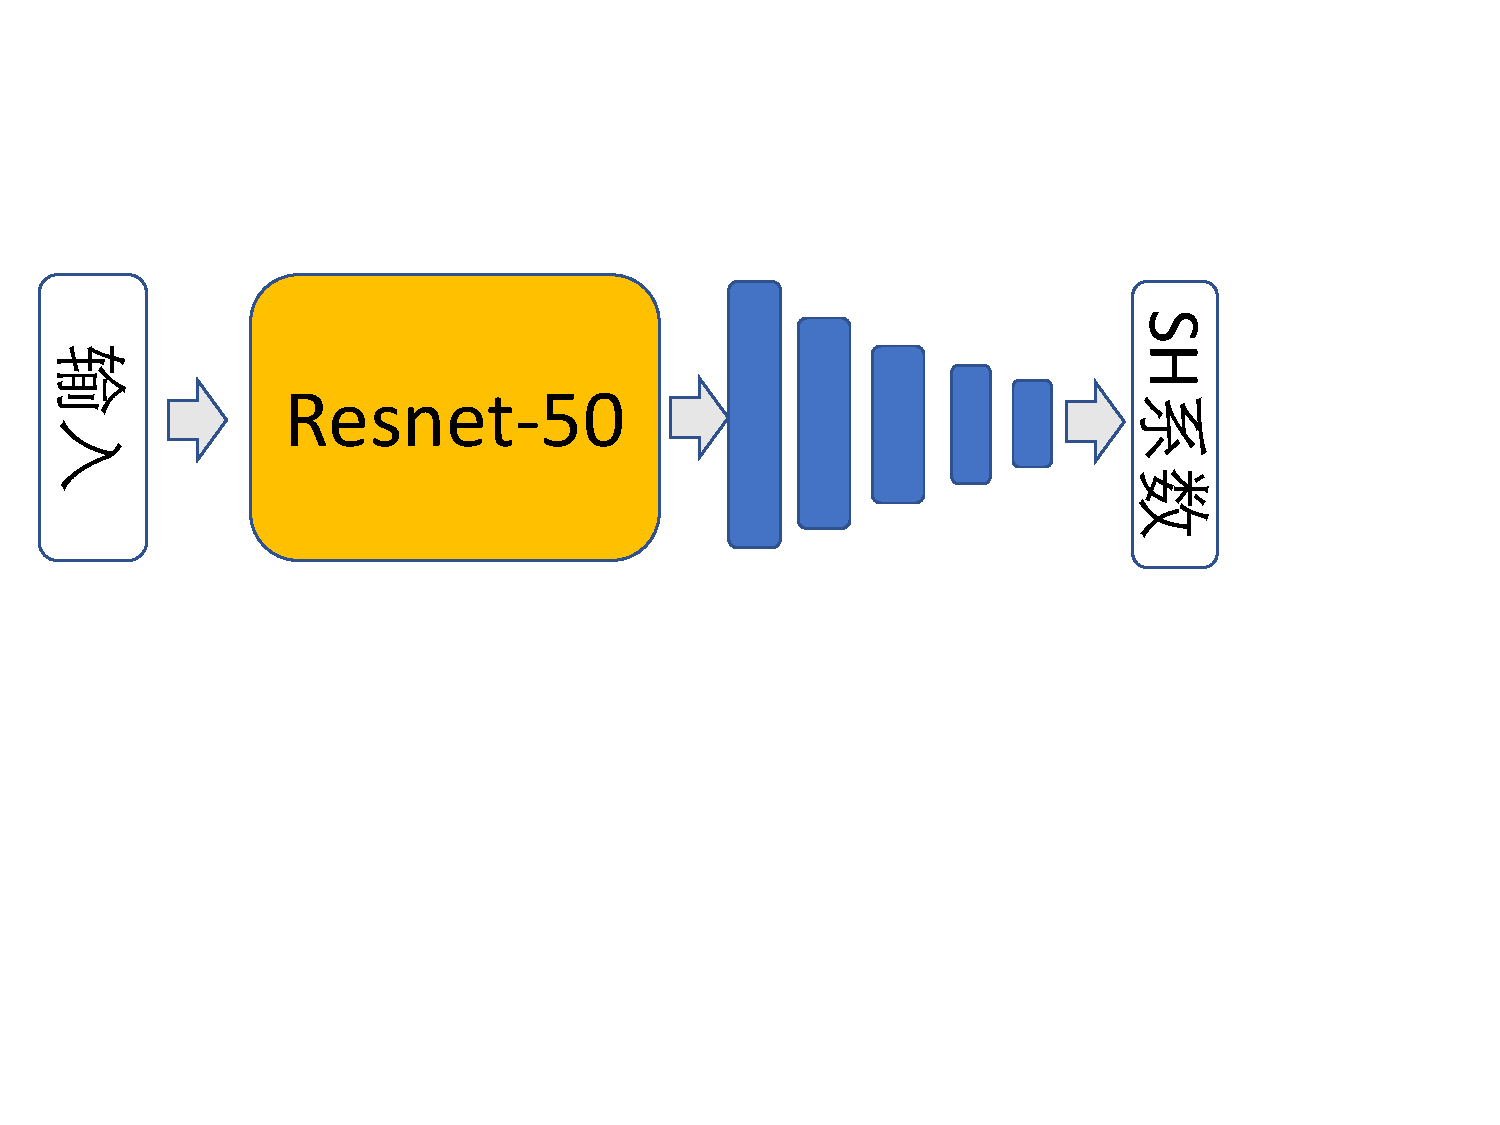
\includegraphics[width=0.6\textwidth]{Img/data-network.pdf}
    \caption[用于评估数据集的卷积神经网络结构]
    {用于评估数据集的卷积神经网络结构。该网络以图片作为输入,输出光照对应的SH系数。网络结构以Resnet-50\cite{he2016deep}为基础,将最后一层pooling层替换为5个全连接层。除最后一层外,每层之后都有BN和RELU激活函数。}
    \label{fig:data-network}
\end{figure}

预测的48个SH系数可以被视为一维向量,向量之间的误差常用L2距离衡量。因此本节实验中使用真实SH系数和估计SH系数之间的均方误差(MSE)作为损失函数,这是一种L2的损失函数。训练使用RMS优化器\cite{tieleman2012lecture},初始学习率为0.0001,衰减系数为0.9,衰减频次为每一个epoch衰减一次。每种实验均在NVIDIA显卡GTX-1080上训练10万步,每步的batch size为16。
\subsection{实验结果:数据的规模对光照估计的影响}
\begin{table}[htbp]
    \centering
    \begin{tabular}{c|c|c|c|c|c}
        \toprule
        训练数  &  100张&  200张&  300张&  400张&  500张 \\ \hline
        RMSE &  0.4502& 0.3108& 0.2161& 0.1892&0.1774 \\
        \midrule
        训练数  &  600张&  700张&  800张&  900张&  ~ \\ \hline
        RMSE &  0.1683&0.1633&0.1621&0.1614 & ~ \\
        \bottomrule
    \end{tabular}
    \caption{
        \label{table:eval-data-size}
        使用不同数量的HDR全景图训练光照估计网络。可以看出,在数据规模较小时,增加训练数据量能够为光照估计带来巨大的提升,但当数据达到一定的规模时,单纯增加训练数据量并不能起到很好的效果。
    }
\end{table}
\begin{figure}[!htbp]
    \centering
    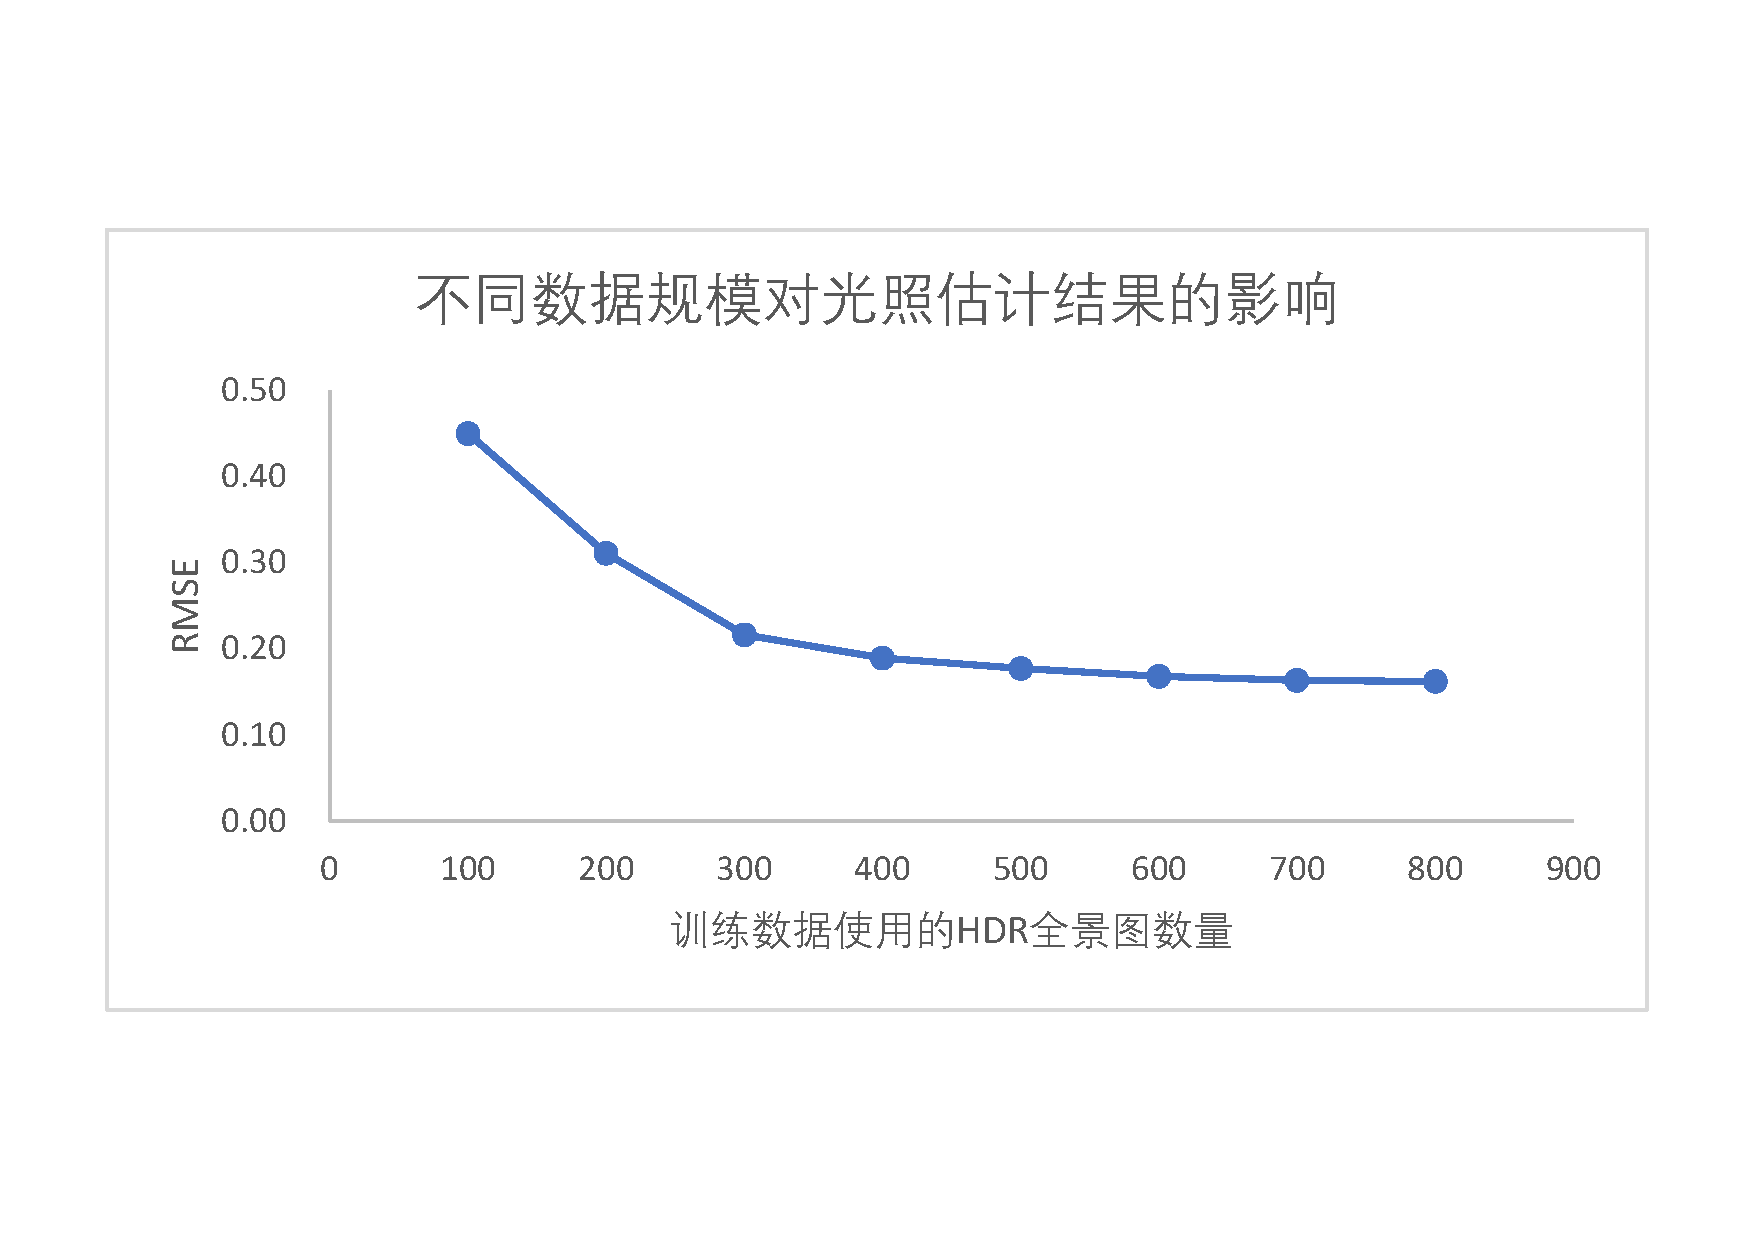
\includegraphics[width=1.0\textwidth]{Img/eval-data-size.pdf}
    \caption[数据规模对光照估计问题影响的趋势图]
    {数据规模对光照估计问题影响的趋势图。可以看出,在数据规模较小时,增加训练数据量能够为光照估计带来巨大的提升,但当数据达到一定的规模时,这种提升达到了饱和,单纯增加训练数据量并不能起到很好的效果,这主要是因为这些场景中包含了一定的重复场景,而在数据中添加更多的重复场景对训练时几乎没有意义的。}
    \label{fig:eval-data-size}
\end{figure}
本实验意图分析不同的数据规模对于光照估计的影响。在划分出验证集后,分别使用100张到900张数据用于训练。在测试时,将验证集中的图片输入到网络中,然后使用估计出的光照渲染一些3D物体,之后将这些结果与使用真实光照渲染的结果进行对比,计算他们之间的均方根误差(RMSE)。它们在验证集的表现如表\ref{table:eval-data-size}和图\ref{fig:eval-data-size}所示。可以看出当数据规模较小时,增加数据对于光照估计效果非常明显,但是当数据规模达到一定的数量时,增加数据所带来的光照估计的提升变得有限。
\subsection{实验结果:数据多样性对光照估计的影响}
\begin{table}[htbp]
    \centering
    \begin{tabular}{c|c|c|c|c|c}
        \toprule
    场景数& 8       &  16  & 32  & 48  & 64 \\\hline
    RMSE &  0.5764 & 0.5277 & 0.4507 & 0.3812 & 0.3117\\
        \bottomrule
    \end{tabular}
    \caption[数据多样性对光照估计的影响]{
        \label{table:eval-data-diversity}
        使用具有不同多样性的数据训练光照估计网络。每一项实验中使用了不同的场景数,但使用的全景图总数是相同的160张。可以看出,当场景数较少时,光照估计的误差很大,并且当增加场景数时,并没有出现像增加数据规模一样的饱和现象。
    }
\end{table}
本实验意图分析数据多样性对于光照估计的影响。在划分出验证集后,分别使用覆盖不同类型的HDR数据训练光照估计网络。它们在验证集的表现如表\ref{table:eval-data-diversity}所示。可以看出增加数据多样性对于光照估计的提升非常明显。在本实验中,用以训练光照估计网络所使用的数据量完全相同,均为320张。他们之间的区别仅仅是数据中所包含的场景种类数、光照条件数不同。从表\ref{table:eval-data-diversity}中可以看到,当仅使用室内或仅使用室外场景时,在验证集上的结果很不理想, 验证集同时包含了室内场景和室外场景,单一场景训练结果的不理想表明室内外场景之间具有很大的差异。
\subsection{实验结果:与其它数据集的对比}
\begin{table}[htbp]
    \centering
    \caption[与现有数据集对比]{
        \label{table:eval-data-previous}
        该实验对比了使用不同的数据集训练光照估计网络时,它们在真实数据集上的表现,从数值结果上可以看出,使用本文构建的数据集在训练光照估计网络时,都优于其它网络。
    }
    \begin{tabular}{c|c|c|c}
        \toprule
    数据集& 本文数据  & 拓展后的SUN360数据 & Laval Indoor\\ \hline
    RMSE &  0.1883 & 0.2437 & 0.2014 \\
        \bottomrule
    \end{tabular}
\end{table}
本实验对比了本文数据集与其它光照估计数据集在光照估计问题中的表现。选取的对比数据集分别是
SUN360\cite{xiao2012recognizing}和Laval Inddor\cite{gardner2017learning}数据集。
这两个数据集是基于深度学习的光照估计方法中最常用的两个数据集,目前多个最先进的(state-of-the-art,SOTA)光照估计方法均是在这两个数据集上进行了训练。其中,SUN360数据集是一个大规模的低动态范围全景图像,为了能将其应用到光照估计问题中,Hold-Geoffroy\cite{hold2017deep}和\cite{gardner2017learning}提出了一种全景数据集上的光照探测方法,将低动态范围全景图像拓展为高动态范围全景图像。在本节实验中,应用了Hold-Geoffroy的方法将SUN360拓展为HDR数据集。Laval Indoor数据集包含了约2000张室内场景的光照,不过其中有大部分的类似的场景(例如同一个场景的多次拍摄),全景图的底部也有大面积的黑色色块(图\ref{fig:laval-indoor}),这些都是会对光照估计问题产生影响的因素。表\ref{table:eval-data-previous}展示了使用不同数据集训练光照估计网络在真实数据集上的表现,图\ref{fig:eval-data-previous}展示了可视的结果。可以看出,无论是数值表现还是可视结果,使用本文构建的数据集在训练光照估计网络时,都优于其它网络。另外,使用SUN360数据训练的光照估计的结果中,在较暗场景中渲染结果与真实值较为接近,但明亮的场景中预测结果与真实值却相差甚远。这也反映了低动态范围全景图本身的局限性,虽然在使用一定的光源探测技术将其拓展为HDR全景图,但这种HDR全景图却很粗糙,限制了其在光照估计问题中的作用。
\begin{figure}[!htbp]
    \centering
    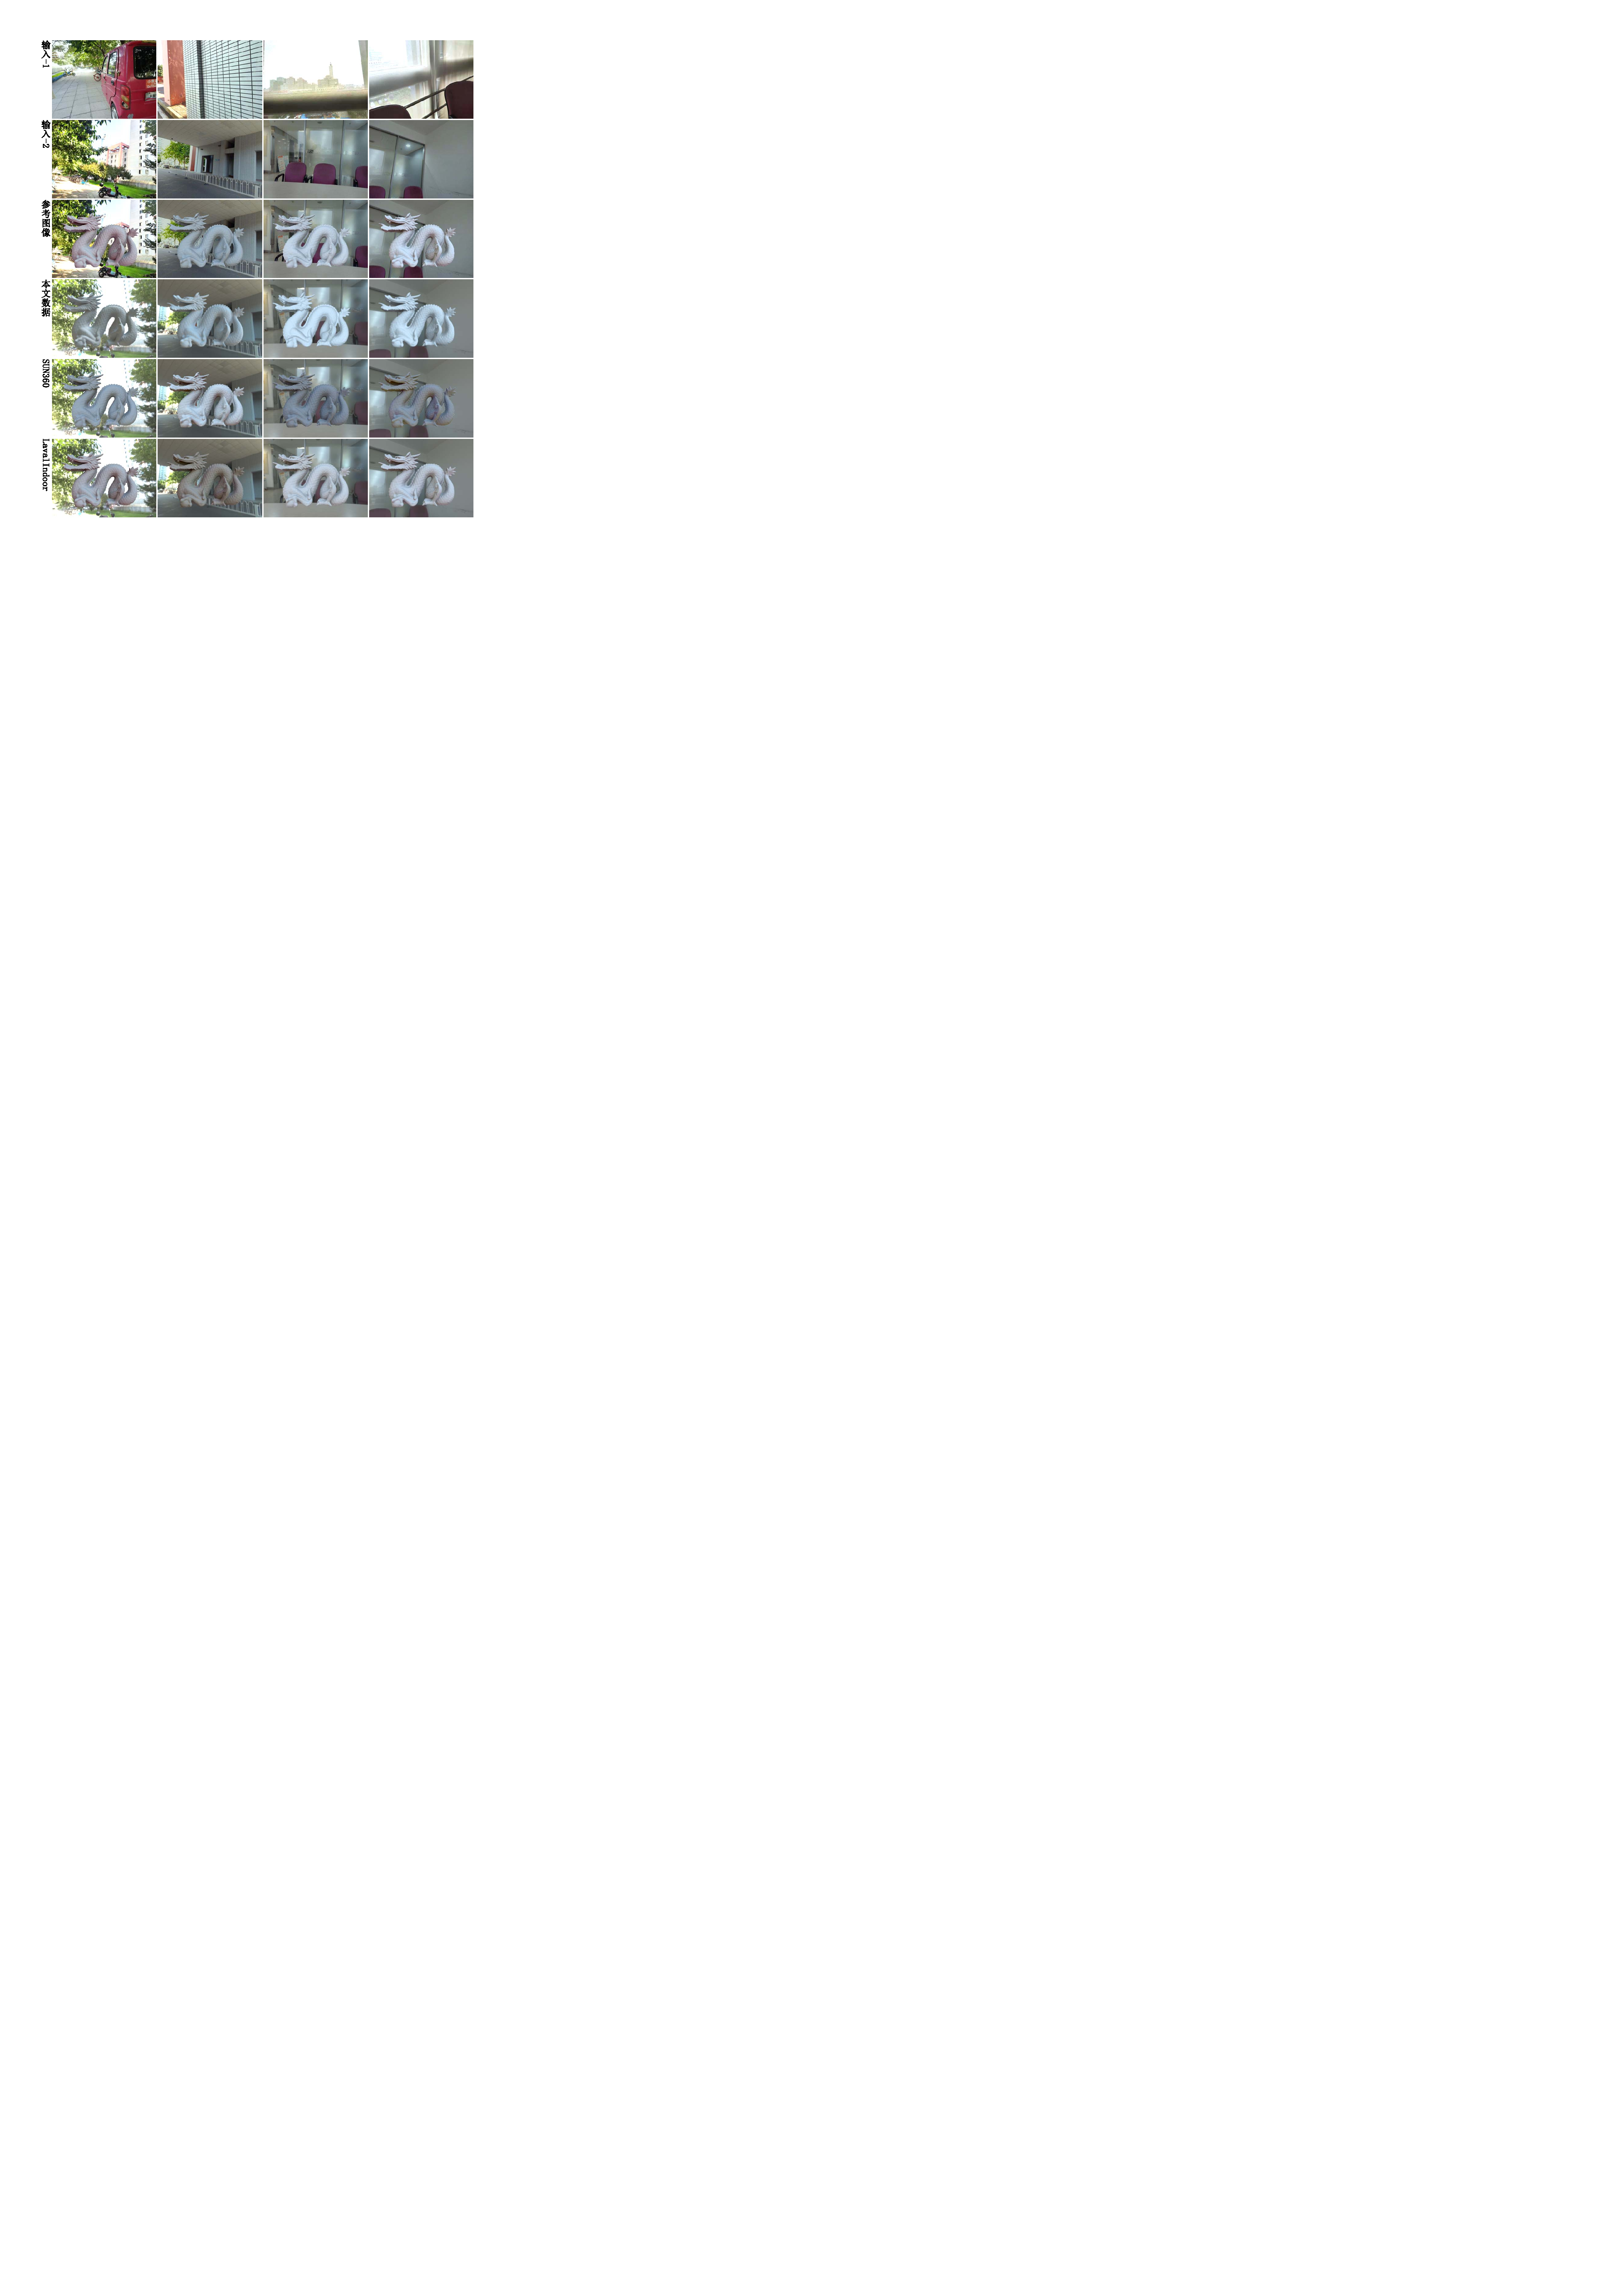
\includegraphics[width=0.98\textwidth]{Img/eval-data-previous.pdf}
    \caption[本文数据集与其它工作的可视化结果比较]
    {使用本文数据集训练的光照估计网络与使用其它数据在可视化结果上的对比。使用本文数据集训练的网络,在室内外场景的结果都明显优于其它两种数据集。另外从结果中可以看出,使用LAVAL数据集的结果在室内场景的表现中较为理想,在室外场景却得到了很差的结果,这是由于laval indoor数据集本身的局限性。使用SUN360数据训练的光照估计网络,在较暗场景中的渲染结果与真实值较为接近(第二列),但明亮的场景中预测结果与真实值却相差甚远(第三、四列)。这也反映了低动态范围全景图本身的局限性,虽然在使用一定的光源探测技术将其拓展为HDR全景图,但这种HDR全景图却很粗糙,限制了其在真实场景光照中的表现。}
    \label{fig:eval-data-previous}
\end{figure}
\begin{figure}[!htbp]
    \centering
    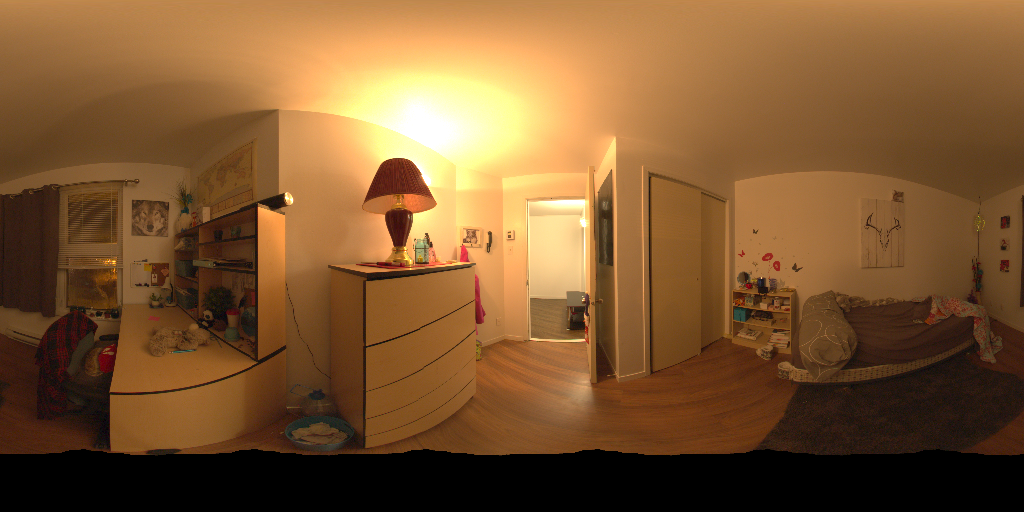
\includegraphics[width=1.0\textwidth]{Img/laval-indoor.png}
    \caption[Laval Indoor数据集中的全景图片]
    {Laval Indoor\cite{gardner2017learning}数据集中的一幅全景图片。由于该数据集在拍摄时将三脚架的部分暴漏在了镜头中,他们在公布数据时选择将这些信息用黑色色块进行了遮挡。虽然经过坐标转换后这些黑色色块的面积没有图中显示的这么大,但依然有可能对光照估计问题造成影响。}
    \label{fig:laval-indoor}
\end{figure}
\section{总结与讨论}
本章介绍了全景图像的两种获取与拍摄方式、存储和预览需要的多种投影方法。根据全景图中颜色的动态范围,可以将全景图分为低动态范围(LDR)全景图和高动态范围(HDR)全景图。LDR全景图与HDR全景图在投影方式、视角范围等并无二致。不过在能表示的亮度动态范围却相差甚远。HDR全景图能够支持大于人类眼睛的动态范围,这使得HDR全景图能够作为真实场景光照的一种表示。

获取HDR全景图通常需要多视角拍摄、多曝光拍摄、全景图拼接、筛选清理、曝光融合五大步骤,本文主要使用了一类可以调节曝光的全景相机,省去了多视角拍摄和拼接的步骤。通过在多类场景、多种光照条件、不同日期和时间的拍摄,本文构建了一个包含550张HDR全景图的数据集,同时额外收集了约500张HDR全景图片,这近千张HDR全景图构成了一个大规模、高质量、具有丰富数据多样性的HDR全景数据。该数据集不仅可以用于光照估计,也可以用于与光照估计相关的其它多种问题。

大规模、多样化的HDR全景数据对光照估计效果的提升需要通过详细严格的实验来验证。本文设计了一系列的对比实验来验证不同的数据规模、数据多样性,以及不同数据集在光照估计网络上的表现。在这些实验中,光照估计网络是在Resnet-50的基础上修改的,网络单张图片作为输入,预测出是光照的球形谐波近似系数。本文设计了三组实验进行对比,分别是数据规模对光照估计网络的影响实验,数据的多样性对光照估计网络的影响实验,以及与其它相关数据集的对比实验。实验结果表明,数据的多样性对于深度学习光照估计方法预测的结果提升很大。在数据规模较小时,增加数据也能够明显的提高光照估计网络的表现。与其它光照估计数据集的对比实验表明,使用本文所构建的数据集训练的光照估计网络有着更好的效果,表明了该数据集在光照估计问题中的优越性。

%% 优点与不足
虽然本文所构建的全景数据集达到了数千张,使用该数据集训练光照估计网络已经能够取得较好的效果,但是该数据集仍然有一定的改进空间,例如可以拍摄更多场景、使用曝光范围更大的全景相机等。此外,从HDR全景图的获取过程可以看出,HDR全景图的拍摄需要对同一场景多次拍摄,因此对于变动的场景无法拍摄为HDR全景图。不过对于光照估计问题来说,该数据集的多样性已经足够保证较好的光照估计结果。